\section{Datenbank / back end / cronjobs}

%% ###################################################################################################
%%   Unterkapitel                                                                                                                                                                              #
%% ###################################################################################################

\subsection{Übersicht}

In diesem Kapitel wird aufgezeigt welche Änderungen an der Datenbank vorgenommen werden und wo diese überall zum Einsatz kommen. Zudem wird aufgezeigt, wie diese zusätzlichen Anwendungen entwickelt wurden. Die Datenbank glich vor der Bearbeitung einem Datenfriedhof. Im jetzigen Zustand werden die Daten die schon geschrieben waren, sowie die neu geschrieben werden aktiv für folgende Aufgaben benutzt:\\
\begin{itemize}
\item API
\item Dreitage Rückschau der verschiedenen Sensoren
\item Historische Daten
\end{itemize}

Die Aufgabe der Datenbank ist es den Umgang der Daten einfacher zu gestalten, sei es in Bezug auf die Aufbereitung der historischen Daten oder aber auch die API, welche einfach erweiterbar sein soll.



%% ###################################################################################################
%%   Unterkapitel                                                                                                                                                                              #
%% ###################################################################################################
\subsection{Datenerfassung}
\subsubsection{Erfassung der Daten des Wetter-Transmitters}
\Diskussionspunkt{- Konfiguration von WeatherDisplay}\newline
\Diskussionspunkt{- Was passiert wenn DB-Eintrag nicht erstellt werden kann}\newline

\subsubsection{Einlesen von Pegel- und Strahlungsmesswerten (Strom to Ethernet)}
\Diskussionspunkt{- wie werden Daten abgerufen?}\newline
\Diskussionspunkt{- was passiert wenn keine Antwort kommt}\newline



%% ###################################################################################################
%%   Unterkapitel                                                                                                                                                                              #
%% ###################################################################################################

\subsection{Datenspeicherung}
\subsubsection{Warum eine Umstrukturierung der Datenbank?}
Die Datenbank ist zur Zeit vor der Umstellung chaotisch und die Namensgebung ist nicht sehr aufschlussreich. Aus diesem Grund wird die Datenbank umstrukturiert. Hierbei soll vor allem die Übersichtlichkeit und Datenverteilung im Vordergrund stehen. Die Daten werden zudem nicht verwendet. Dies ist sehr schade, da es auch für vergangene Daten Anwendungen gibt, bspw. könnten Benutzer zurück schauen um zu sehen wie das Wetter vor einem Jahr war. Hierfür wird eine Seite mit einer solchen Anwendung erstellt.

\subsubsection{Vorgaben}
Bei der Entwicklung einer Datenbank müssen verschiedene Punkte vorher klar sein. Zum einen welche Datenbank steht zur Verfügung und welches Datenmodell bildet diese. Der wichtigere Punkt der beiden Fragen ist welches Datenmodell wird benutzt denn es bestehen folgende Arten von Datenmodellen:
\begin{itemize}
\item relationale DB
\item hierarchisches Datenmodell
\item Netzwerkdatenmodell
\item Objekt relationale Datenbank
\end{itemize}

Im Falle der zu bearbeitenden Datenbank ist steht eine MariaDB mit einer relationalen Struktur zur Verfügung. Die relationale Datenstruktur heisst so, weil es in diesem Fall der Modellbildung sich überlappende Spalten geben kann.\cite{IntroductionToRelationalDatabases:MariaDB} Hiermit werden die verschiedenen Tabellen welche entwickelt werden auf beliebige Weise durch dieses Feld verknüpft. Im Falle der neuen Datenbank wird es die Spalte datetime sein, dazu aber später mehr.\\

\subsubsection{Methodik}
Nachdem die Vorgaben klar sind kann die Datenbank entwickelt werden. Hierbei kann es verschiedene Methoden geben. Im Falle dieser Datenbank wurde entschieden nach einer Methode mit vier verschiedenen Phasen zu nehmen. \cite{Datenbanken:GrundlagenUndEntwurf:VeikkoKrypczyk} Dieses Vorgehen sieht folgendermassen aus:
\begin{itemize}
\item Externe Phase (Ermittlung der Informationsstruktur)
\item Konzeptionelle Phase (ER-Modell)
\item Logische Phase (relationales Datenmodell)
\item Physische Phase (Erstellung des Datenmodell)
\end{itemize}

Diese vier Phasen führen vom Beginn der Enwicklung bis zum Endprodukt und werden im nächsten Kapitel erklärt sowie gleich umgesetzt.
\subsubsection{Neugestaltung der Datenbank}
\textbf{Externe Phase}\\
In der externen Phase gilt es herauszufinden, welche Daten aus der realen Welt dargestellt werden sollten, sowie das Problem darzustellen. Das Problem bei dieser Arbeit sind die Menge an Daten, vor der Bearbeitung der Datenbankt fällten Stündlich 60 Einträge mit 65 Datenpunkte an. Dies ergab über die 3 Jahre an der Die Datenbank mehr oder weniger minütlich gefüllt wurde 1143847 Einträge. Dieser ganze Satz an Daten gilt es zu optimieren und die zukünftigen Einträge auf die wichtigsten zu minimieren. Dies ging auch aus der Diskussion mit dem Spezialisten hervor, welcher einige Ansätze, für eine neu Organisation aufgezeigt hat hervor. Die Umstrukturierung der Datenbank sieht folgende Massnahmen vor. Die Tabelle wx data, beinhaltet die Daten des Wettertransmitters wird möglichst in ihrem Zustand belassen. Es werden einzig die Spalten, welche immer eine 0, 100 oder ein NULL beinhalten gelöscht. Die restlichen Daten werden in eine neue Tabelle überführt. Die Tabelle tblwellen, beinhaltet den Pegel wird gelöscht. Dafür kommt eine neue Tabelle welche alle Daten der externen Sensoren beinhaltet. Zudem wird eine historische Tabelle erstellt, welche die Daten aus den beiden vorher erwähnten Tabellen zusammengesetzt wird erstellt. Diese wird für die Seite mit historischen Daten weiterverwendet. Um die historische Tabelle ohne ausfälle zu füllen wird eine Tabelle entstehen, welche alle Zeitstempel bis zum Jahre 2030 beinhalten. Welche Datenpunkte übernommen werden kann aus dem Anhang \Diskussionspunkt{AUF ANHANG VERWEISEN} entnommen werden.\\

\textbf{Konzeptionelle Phase}\\
Nachdem die externe Phase abgeschlossen ist und entschieden ist, welche Datenpunkte für die API sowie die neue Webseite relevant sind kann mit der konzeptionellen Phase begonnen werden. In dieser geht es darum die in der vorhergehenden Phase in ein Konzept zu überführen. Bei der Erstellung einer Datenbank besteht die Möglichkeit ein ER-Modell zu entwickeln. Ein ER-Modell zeigt die verschiedenen Beziehungen unter den Tabellen auf, welche Entitäten eine Datenbank hat und welche Attribute eine Datenbank beinhaltet.\cite{FrankGeisler2011mitpu} Um diese Punkte zu definieren muss klar sein welche Attribute eine Tabelle hat. Wird eine Tabelle mit allen Attribute erstellt oder mehrere logisch aufgeteilte Tabellen? Die Daten werden in Zukunft in drei Tabellen aufgeführt, welche je ein eigenes ER-Modell beinhalten.\\

Beim ER-Modell für die Daten des Wettertransmitters, Bild \ref{img:ER_Modell Wettertransmitter},  beinhaltet jeder Zeitstempeleintrag, das bedeutet jede Minute des Tages die Daten des Wettertransmitters. 

\begin{figure}[h!]
  \fbox{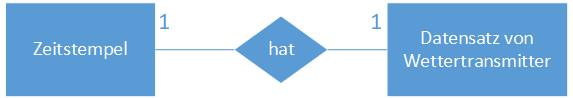
\includegraphics[width=\textwidth-2\fboxsep-2\fboxrule]{img/ER_Modell_Wettertransmitter}}
	\centering
	\caption{ER-Modell der Daten vom Wettertransmitter}
	\label{img:ER_Modell Wettertransmitter}
\end{figure}

Dasselbe, wie beim ER-Modell für den Wettertransmitter, gilt auch für die externe Sensoren, wie in Bild \ref{img:ER_Modell externe Sensoren} zu sehen ist. 
\begin{figure}[h!]
  \fbox{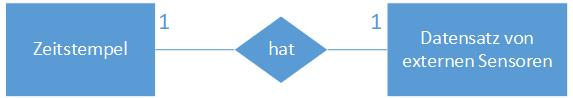
\includegraphics[width=\textwidth-2\fboxsep-2\fboxrule]{img/ER_Modell_externe_Sensoren}}
	\centering
	\caption{ER-Modell der externen Sensoren}
	\label{img:ER_Modell externe Sensoren}
\end{figure}

Beim Modell der historischen Daten sieht das ganze anders aus, siehe Bild \ref{img:ER_Modell historische Daten}. Hier beinhaltet jeder Zeitstempel den Median sowie die Extremwerte der Daten vom Wettertransmitter und die der externen Sensoren.

Ein ER-Modell für die Datumstabelle ist nicht notwendig, da diese nur die Daten beinhalten und sonst keine weiteren Daten enthalten.

\begin{figure}[h!]
  \fbox{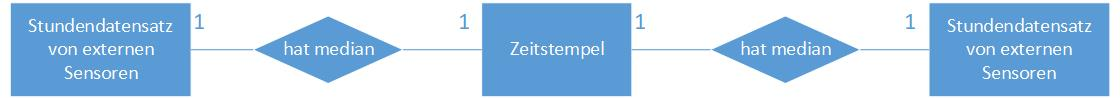
\includegraphics[width=\textwidth-2\fboxsep-2\fboxrule]{img/ER_Modell_historisch}}
	\centering
	\caption{ER-Modell historische Daten}
	\label{img:ER_Modell historische Daten}
\end{figure}

\textbf{Logische Phase (relationales Datenmodell)}\\

In der logischen Phase geht es darum das ER-Modell in ein relationales Datenmodell zu überführen. Hierbei wird entschieden welches die primärschlüssel der einzelnen Tabellen sind und wie diese zusammenhängen. Im zweiten Schritt wird, wenn nötig eine Normalisierung vorgenommen. Das relationale Datenmodell unterscheidet sich in der Struktur nicht gross vom ER-Modell. Der grosse Unterschied hierbei ist jedoch, dass die Primärschlüssel, sowie die verschiedenen Datentypen entschieden werden. Die sogenannten Schlüssel sind im relationalen Datenmodell auch ein wichtiges Merkmal. Die Schlüssel sind entscheidend beim zukünftigen Datenbankeintrag, beispielsweise wenn zu einem bestimmten Zeitpunkt nur ein Datensatz vorhanden sein kann. In diesem Fall wird ein Zeitstempel als Primärschlüssel definiert. Weitere Möglichkeiten wäre auch ID, welche automatisch hochzählt. Für die Datenbank des Wetterdaten, soll von einem Zeitstempel gebraucht gemacht werden. Dieser wird jedoch nicht in der Datenbank generiert, sondern beim Auslesen der Daten. D.h. der Datentyp ist Datetime, da ansonsten der Zeitstempel von der Datenbank übernommen wird. Für die historische Tabelle wird der Primärschlüssel aus der DateMaster Tabelle entnommen. So kann sichergegangen werden, dass wenn in die Tabelle tblextsensors und tblwettertransmitter keine Daten geschrieben werden dennoch ein Eintrag in die historische Tabelle möglich ist. Das relationale Datenmodell kann aus dem Anhang \Diskussionspunkt{AUF ANHANG VERWEISEN} entnommen werden.\\ \Diskussionspunkt{Was ist normalisierung}\\


\textbf{Physische Phase (Erstellung des Datenmodell)}\\

In der physischen Phase wird das Konzept, welches in den vorherigen Schritten erstellt wurde umgesetzt. Bei der Umsetzung entstanden anschliessen einige Herausforderungen. Dazu aber später mehr. Die drei konzipierten Tabellen konnten wie gewünscht umgesetzt werden. Der Code für die Umsetzung der Tabellen kann aus dem Anhang entnommen werden.\\
Bei der Umsetzung wurde zudem noch entschieden eine vierte Tabelle zu erstellen, tblmisc, diese beinhaltet die Daten, welche von einem dritten Angeboten werden. Im Falle der Wetterstation beinhaltet diese die Sturmwarnung. Auch diese Tabelle kann mit weiteren Spalten ergänzt werden 
Das Problem bei der Umsetzung war, das die historische Tabelle welche aus den beiden Tabellen tblwettertransmitter und tblextsensors. Bei der Query um die Extrema und Mediane zu erstellen stellte sich heraus, dass die drei Tabellen, tblwettertransmitter, tblextsensors und DateMaster zu gross sind um es direkt mit einem LEFT JOIN umzusetzen. Deswegen musste hier auf eine sogenannte View zurückgegriffen werden. Der VIEW beinhaltet die minuten Daten der vergangenen 48 Stunden aus den zwei Tabellen tblwettertransmitter und tblextsensors. Dieser VIEW wird zudem für die Graphen auf der Webseite verwendet. 

\subsection{Datenbanksicherheit}
\subsubsection{Speicherplatz}
Vor dass sich Gedanken um die Datensicherheit gemacht werden, sollten die die Bedingungen an Speicherplatz klar sein. Während der Laufzeit werden grosse Mengen an Daten in die Datenbank geschrieben, vor der Neukonzipierung werden täglich 1440 Datensätze gespeichert. Dies bedeutet jede Minute einen Datensatz. Ein Datensatz beinhaltet 65 Einträge, die gesamte für die Arbeit relevante Datenbank igwetter wettertest benötigt 323.17  Mb. Nur schon die Tabelle wx data, diese beinhaltet die Minutenwerte des Wettertransmitters, benötigt stand 1.3.18 311.94 Mb, daraus erfolgt das ein Datensatz ca 0.025 Mb benötigt. Für den Speicherplatz, welcher 50 Gb bietet, stellt dies kein Problem dar, da wenn man die Zahlen hochrechnet genügend Platz für die kommenden 45 Jahren.\\


\subsubsection{Angriffssicherheit}

Bei der Recherche nach Datenbanksicherheit taucht immer wieder das Wort Injection auf. Laut den OWASP top 10, eine Liste welche die wichtigsten Schwachstellen aufzeigt, ist die SQL-injection in 2017 auf dem Platz 1. Was ist den eigentlich SQL Injection? SQL injection ist eine Methode eine Datenbankabfrage so zu manipulieren, dass der Angreifer im schlimmsten Fall auf die gespeicherten Daten des Administators kommt. Ein anderes Beispiel wäre, dass der Angreifer an die Daten der Benutzer eines Online-Shops mit Kreditkartendaten oder ähnlichen sensitiven Daten kommt.
Weitere Fragen die auftauchen bei der Suche nach Datenbanksicherheit sind:
\begin{itemize}
\item Was für Arten von Daten beherbergt die Datenbank?
\item Hat es sensitive Daten?
\item Ist die Datenbank überhaupt ein potentielles Angriffsziel?
\item Wer sind die Benutzer der Datenbank?
\end{itemize}

Bei der Wetterstation Arbon, bestehen keine persönliche oder Sicherheitsrelevante Daten in der Datenbank. Somit ist diese aus sicht eine potentiellen Angriffes eher uninteressant. Dennoch sollten die Daten hinreichend geschützt sein, da es vorallem schade wäre wenn die Daten verloren gingen. Andererseits aber auch das kein Missbrauch vom Server gemacht werden kann.

Die Zugriffe auf die Datenbank sind so gestaltet, dass nur Serverseitig darauf zugegriffen wird. Die Darstellung der Anzeigen auf der Webseiten werden über die API erstellt. Die API wiederum ist so aufgebaut, dass ein PHP-Skript auf dem Server die Daten aus der Datenbank abgreift und sie richtig formatiert. Somit kann sichergegangen werden, dass keine SQL-Infection möglich ist. Wie im Kapitel \Diskussionspunkt{Kapitel Erwähnen} erwähnt, müssen die Daten für das Tableau manuell übertragen werden. Dies bedeutet auch für die historische Seite ist kein Datenbankzugriff notwendig. 

\subsubsection{Backup}

Um die Datenbank auch gegen einen allfälligen Datenverlust zu sichern ist ein Backup von wichtiger Bedeutung. Deswegen ist das Backup ein weiterer Aspekt gegen den Verlust von Daten. Hierbei sind folgende Fragen relevant:
\begin{itemize}
\item Welche Daten sollen gesichert werden?
\item Wie oft sollten die Daten gesichert werden?
\item Wie bzw. wo sollte das Backup gelagert werden?
\end{itemize}

Da alle Daten in der DB gleich relevant sind sollten auch alle so behandelt werden und im Backup vorhanden sein. Dabei muss aber entschieden werden, ob ein tägliches Backup Sinn machen würde. Bezüglich des Speicherplatzes und des Aufwands, da die Wetterstation von einem Verein betrieben wird, ist es wichtig den Aufwand mit dem Ertrag zu vergleichen.Zusätzlich sollte das Backup nicht auf dem Server des Providers gespeichert werden, da wenn etwas schief geht mit dem Server die Daten auch weg sind. Deswegen ist es wichtig auch ein "externes" Backup zu erstellen. Hostpoint bietet für das Backup verschiedene Varianten:
\begin{itemize}
\item Cronjob
\item Backup auf Knopfdruck
\item Kostenpflichtige Wiederherstellung aller Daten
\end{itemize}


Um den Aufwand klein zu halten wird empfohlen ein monatliches Backup mit der Backup Funktion auf Knopfdruck zu erstellen und dieses auf einer Festplatte zu speichern, siehe Bild \ref{img:Backup_Funktion} 
\begin{figure}[h!]
  \fbox{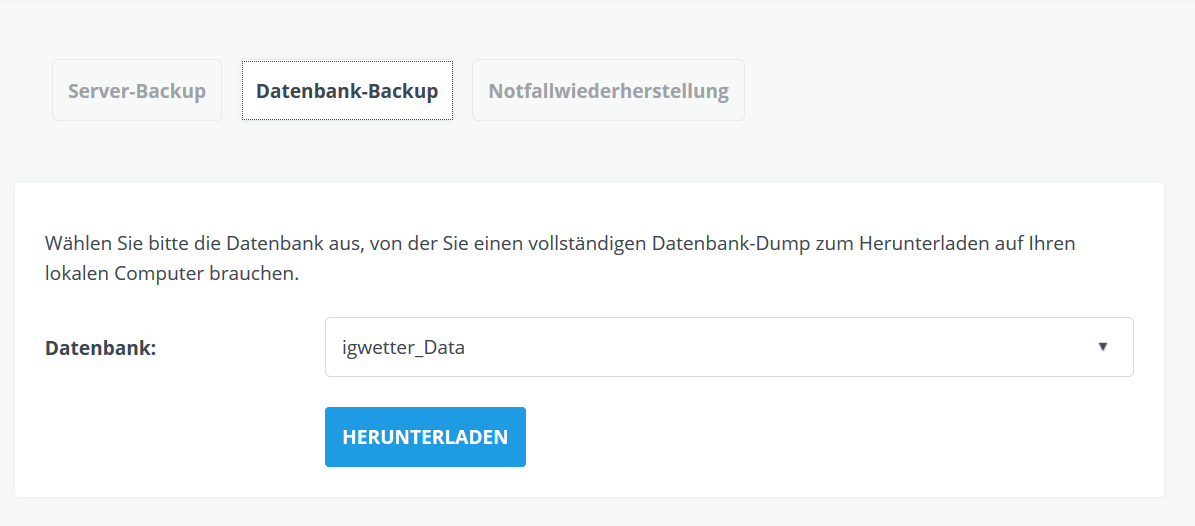
\includegraphics[width=\textwidth-2\fboxsep-2\fboxrule]{img/Backup_funktion}}
	\centering
	\caption{Backup auf Knopfdruck von Hostpoint}
	\label{img:Backup_Funktion}
\end{figure}
Sollte trotzdem mal das Backup nicht funktionierten oder vergessen gegangen sein, kann auf den Hostpoint-Service \ref{img:Notfallwiederherstellung}  züruck gegriffen werden. Diese erstellen selber ein tägliches Backup, welches für 100 Franken wieder eingespielt werden kann.
\begin{figure}[h!]
  \fbox{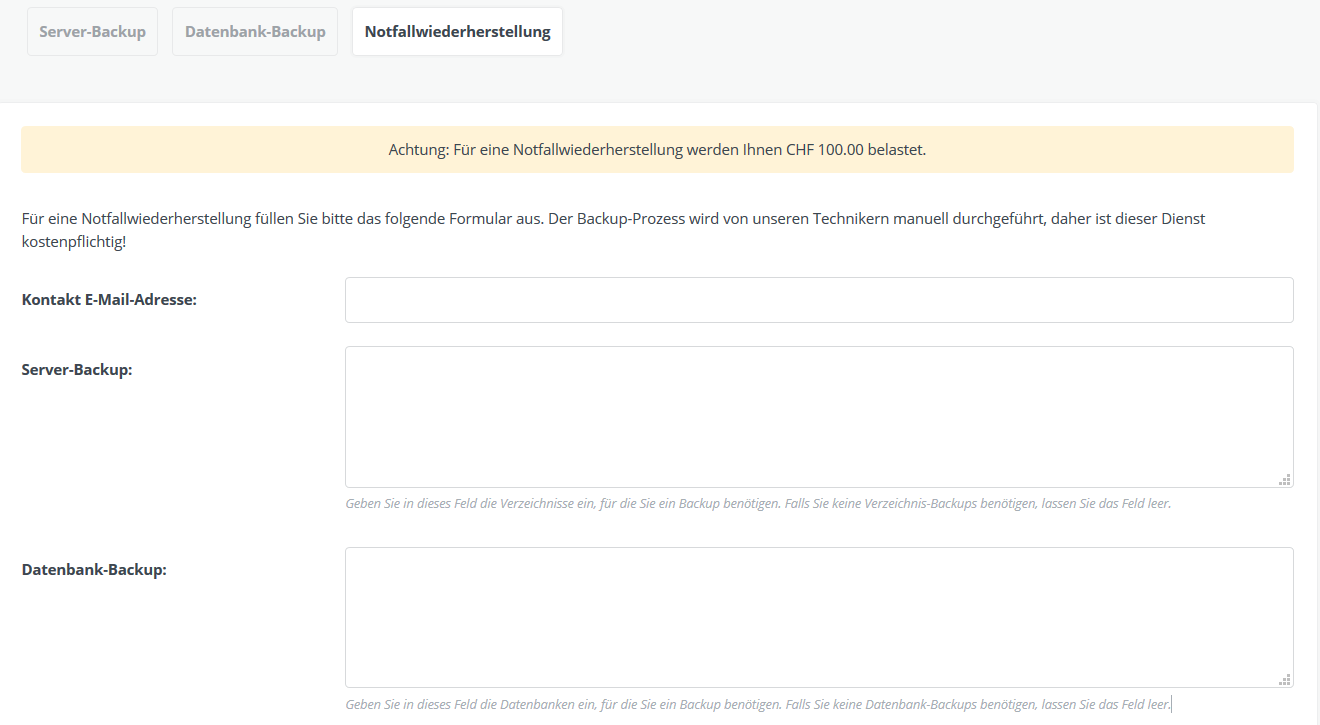
\includegraphics[width=\textwidth-2\fboxsep-2\fboxrule]{img/Notfallwiederherstellung}}
	\centering
	\caption{Notfallwiederherstellung von Hostpoint}
	\label{img:Notfallwiederherstellung}
\end{figure}
Somit können sich, davon ausgehend, dass Hostpoint einen guten Job macht Kosten für bspw. ein Cloudaccount gespart werden.

%% ###################################################################################################
%%   Unterkapitel                                                                                                                                                                              #
%% ###################################################################################################

\subsection{Datenarchivierung}

Bei der Datenarchivierung geht es vor allem darum, wie mit den vergangenen Daten umgegangen wird. Da nach der Umgestaltung eine neue Tabelle tblhistorical entstanden ist, bestehen zwei Möglichkeiten um mit den Daten umzugehen. Allerdings ist eine Anforderung an die tblhistorical, dass diese nur Stundenwerte beinhaltet. Konkret bedeutet dies, dass aus den Werten einer Stunde der Median und die Extremwerte extrahiert werden. Auf die zwei Möglichkeiten bezogen bedeutet dies folgendes: \\
Die erste Variante ist die historische Tabelle stündlich zu füllen mit einem Datensatz und bei den beiden Tabellen tblwettertransmitter, sowie tblextsensors die Werte wieder zu löschen. Dies würde bedeuten, dass schlussendlich nur die historische Tabelle vorhanden ist um in die Vergangenheit zu schauen.\\
Die zweite Variante ist, die historische Tabelle stündlich zu füllen, jedoch die Tabelle des Wettertransmitters und der externen Sensoren gefüllt zu lassen mit den historischen Minuten Werte.\\
Da beim Server der Speicherplatz kein ausschlaggebender Punkt ist, wurde für die zweite Variante entschieden. Diese hat zudem noch den Vorteil, dass die Minuten Werte der Vergangenheit noch vorhanden sind, sollte eine zusätzliche Anwendung hierfür entstehen.


%% ###################################################################################################
%%   Unterkapitel                                                                                                                                                                              #
%% ###################################################################################################

\subsection{Funktionsüberwachung mit Mail-Service}

Um die Funktion der Software zu gewährleisten, sollte bei einem Absturz der Verantwortliche für die IG bei der IG benachrichtigt werden. Folgende Funktionen müssen bei einem Absturz eine Meldung geben.
\begin{itemize}
\item Einlesen Sensordaten extern
\item Einlesen Wettertransmitter Daten
\item Erstellung der stündlichen historischen Daten
\end{itemize}
Die Aufgezählten Funktionen werden alle bis auf das Einlesen der Wettertransmitter Daten über einen Cronjob ausgeführt. Für die Cronjobs bietet Hostpoint den Service, dass bei einem print() die Ausgaben per Mail an eine bestimmte Mailadresse gesendet werden, im Beispiel \ref{lst:printfunction}. Für das Einlesen der externen Sensordaten sieht der Mailservice folgendermassen aus. Können einer der Webservices vom \Diskussionspunkt{A/E Wandler} nicht erreicht werden, wird die folgende Mail generiert:\\
Es ist ein Problem mit (der Temperatur, dem Pegel, dem Strahlungssensor) aufgetreten. Exception: ...\\
Je nach Sensor wird dieser genannt und das Problem welches aufgetreten ist. Für die Erstellung der historischen Daten und dem einlesen der Wettertransmitter Daten sieht die Lösung ähnlich aus. Jedoch werden diese beiden im gleichen Cronjob, dem erstellen der historischen Daten kontrolliert. Zuerst wird kontrolliert ob alle 60 Einträge der letzen Stunde vorhanden sind. Ist dies nicht der Fall, würde es bedeuten, dass das WeatherDisplay, welches die Daten des Transmitters aufbereitet, abgestürzt ist und neu gestartet werden muss. Das zweite was in diesem Cronjob kontrolliert wird, ist dass Kontrolliert werden muss ob die Daten in die historische Tabelle geschrieben sind. Die beiden Meldungen sehen dann so aus:\\
Bitte starte das WeatherDisplay neu, es wurden nur (Anzahl Datensätze) Daten geschrieben.\\
Die historischen Daten können nicht geschrieben werden, es besteht folgendes Problem (Exception).\\

Um diese Funktionen zu erstellen wird Gebrauch gemacht vom try, except Verfahren in Python. Zu Beginn wird der Code im try ausgeführt, tretet keine exception auf wird das except übersprungen und der anschliessende Code ausgeführt. Tritt aber während dem try eine exception auf, wird der Code unterbrochen und der im except weitergeführt. Anschliessend wird der Code nach dem Exception Handling ausgeführt.\cite{ThePythonTutorial8.ErrorsAndExceptions:Python}

\begin{lstlisting}[label=lst:printfunction,caption=Beispiel für print Funktion, language=Python, style=py]
except Exception as e:
    print "Es ist ein Problem mit der Strahlungs Abfrage aufgetaucht: "
    print e
\end{lstlisting}

%% ###################################################################################################
%%   Unterkapitel                                                                                                                                                                              #
%% ###################################################################################################
\subsection{Cron-Jobs}
\Diskussionspunkt{- Printscreen cronjobs-Konfig auf Hostpoint}\newline


%% ###################################################################################################
%%   Unterkapitel                                                                                                                                                                              #
%% ###################################################################################################
\subsection{Problematik Zeitumstellung}



